\documentclass{project}
\usepackage[pdfauthor={C. P. Marriott},pdftitle={Software Engineering Group Project, Project Plan},pdftex]{hyperref}
\usepackage[pdftex]{graphicx}
\usepackage{pdfpages}
\hypersetup{colorlinks=false,pdfborder={0 0 0}}
\begin{document}
\title{Software Development Life cycle}
\subtitle{End of project report}
\author{Tom Reed, Matt Whitmore, Dave Clark, Silhab Csoma, Mike Steel, Chris 'Tux' Lloyd, Aleksandra Badyda, Samuel Jackson, Chris Marriott}
\shorttitle{End report}
\version{1}
\status{draft}
\date{2013-02-07}
\configref{SE.17.DS.01}
\maketitle
\tableofcontents
\newpage

\includepdf[pages={4-22}]{DesignDocument.pdf}

\section{Management Summary}
This project has managed to achieve 25/27 of the functional requirements it was aiming to complete. See (cite requirements doc) for list of functional requirements. The only two that were not managed to be completed on time were, monster aging and server to server. The mosters ageing requirement, although not implemented, there was a formula that we had that worked. Given a bit longer on the project I believe we could have got the monster ageing working. The server to server side however was a bit further off. Silhab Csoma had a look at the server to server but due to the change in requirements and internet down time there was not time to implement server to server.
\\
All the documents have been worked on thoroughly and I feel that they are up to a more than reasonable standard.
\\
\\
A few difficulties got in our way during the development of the system. One of these issuses was the change of requirements. Originally it was specified that the monster battle and breed would be offered up or requested but as the deadline approached the functional requirements were changed to specify that breed and battle requests had to be offered. This meant that part of the system had to be redesigned which took time off working on bugs and other functional requirements. 
\\
\\
Another major issue that arose was that there was internet downtime in the week before the deadline. This caused several issues, the first of which was the inability to test the system properly. This lead to work on the system being slowed down and thus resulted in a less complete system. It also meant more two of the coders(Sam Jackson and Chris 'Tux Lloyd) had to put in more hours to complete what was necessary to get a functional and bug free program. 
The second issue the internet downtime caused was a loss of work as when uploading the latest copy to git there was an error in doing so. We then tried to access the project which was stored on the M: drive however, this was unaccessable. We decided to leave the university grounds and head down into town to find somewhere with a working internet connection. Here the two coders managed to get access to the temporarily back up internet and M: drive and obtain a copy of the latest code. From here it was then uploaded to GitHub with an issue that meant the latest CSS code would be Lost. This meant Aleksandra Badya had to put more work into finishing of the design of the system.  
\\
\\
The team preformed outstandingly overall. However special credit has to go to Chris 'Tux' Lloyd and Samuel Jackson as they worked perfectly as a team. Between them they managed to sort out a large quantity of the bugs and get a large chuck of the system operational. The rest of the team fulfilled there roles and more, they managed to do what was asked of them and more. 

\section{Historical account of project}
The main events of this project were as follows;
The first main event that happened was the meeting of the group. This is classed as a main event as we did not all know each other so we decided to meet up and get to know one another so we would find it easier to work with each other. This proved a good idea and thankfully every team member seemed to get on well with each other. We also assigned tentative roles to team members.
\\
Next we started work on creating the system and project plan document. During this document creation we had weekly meetings and regular reviews of the document. The system was also starting to take shape at this time with parts started to be developed. 
\\
After the project plan document we moved onto the test specification document and designing the web interface. Again with this document we also had weekly meetings and reviews of the documents being produced. As well at this point in the project team members were getting more familiar with using \LaTeX to standardise documents and github for version control. System continued to develop at this point.
\\
Work then began on the design specification document for the system and getting a prototype ready for demonstration. The whole group worked briliantly on documenting, testing and implementing all aspects of the system. After this we worked on improving the documents and the system up to a standard that would be ready to hand in.
\\
The final stage of this project was 'testing and implementation week' where the project was developed into the best state it could be. Here Samuel Jackson and Chris 'Tux' Lloyd managed to get more or less the whole system working even after internet down time cause issues with the project as well as a change of functional requirement. The documentors helped by testing the system and reporting any issues/bug so they could be fixed. Then the final document was produced which is a combined working of all the documents that have been worked on.
\\
The team worked very well with each other communicating when needed and completing tasks set for them. 

\section{Final State of project}
The final state of the project is that 25/27 of the functional requirements were fulfilled. The only two requirements that were not fulfilled were the monsters ability to age and the ability to connect server to server. 

This should give a summary of which parts of the project are perceived as correct and
which are not. It is as well to be as accurate as possible here - more marks will be deducted for problems that are
not declared but are detected by the markers than for problems that are declared in the final report. As well as
missing or erroneous features in the software, known problems with documents should be included here.

\section{Performance of each team member}
\subsection{Tom Reed}
Tom's duties as Q.A. Manager were to manage other documentors and delegate documenting tasks where he felt appropriate. He preformed brilliantly especially as the deadline approaced, he assigned tasks well and made sure they were completed. He also kept Christopher Marriott(Project Manager) up to date on goings and asked for more work when finished allcurrent work. He was an essential part of the team. 

\subsection{Chris 'Tux' Lloyd}
Tux preformed outstandingly. His time and effort put into the code was brilliant and he worked well with the rest of the team. He informed people of changes and explained things clearly. He worked especially well in tandem with Samuel Jackson. He put countless hours of work into the project and helped solved numerous bugs. Tux worked on the server side of things, getting the connectivity working with Samuel Jackson and Silhab Csoma side of code.

\subsection{Samuel Jackson}
Sam's preformance was outstanding. Not only was he vital in the functionalality of the overall system but on occasion preformed as a brilliant project leader when Christopher Marriott was away. His main role was to work on Javascript for the system. He helped get the system up and running and helped keep the team on track with their roles. He also put in a large amount of time into the project.

\subsection{Silhab Csoma}
Silhab's work on data structions and work on algorithms was essential to the working of the system. Without these in place there would be no way of storing monster and user info. She worked well in a team and completed all tasks set for her.

\subsection{Alexsandra Badya}
Alex worked well in the team. She provided vital support to the team with git did great work with the html and css. She also worked well as deputy Q.A. manager when Tom Reed was away. The team were kept up to date with duties they had to complete. She performed very well on the whole project.

\subsection{Dave Clark}
Dave was a very good documentor in all areas. He mostly focused on Tux's server side documentation however he also work on other documentation. He also helped find bugs with in the system and inform people of what they were. Other areas he worked on were the database diagram, methodology and reviewing functionality. He also did the minutes for several of the team meetings.

\subsection{Mike Steel}
Mikes main duty was to document Silhab's work. He performed well within the team and helped in other areas. He helped out on the testing side of the system and fixing the \LaTeX  documents. He also produced the risk assessment and designed the monster mash logo that we use on the main system webpage.

\subsection{Matt Whitmore}
Matt's job was to document and test Alex's HTML and CSS. He completed all tasks on time and worked well with the team. He also helped out on the testing of the system and found some bugs of which he informed the appropriate people. 

\subsection{Christopher Marriott}
Chris' main role was project manager. As project manager it was Chris' duty to assign tasks to other team members, review documents and check that people are completing their tasks. He communicated to the group regularly and organised meetings, he also on occasion took the minutes.  

\section{Critical evaluation of the team and project}
\subsection{Team performance}
The teams performance was brilliant. A few team members also went above and beyond the call of duty to get the system more or less fully functional. Everyone knew their role and were happy with the tasks they were set. If anyone had a problem they spoke to the appropriate person and got it resolved reasonably quickly. Everyone did their roles excelently and fulfilled all that was required and more. Each member of the team communicated clearly with other team members and kept up to date with what had been done and what had not. Each team member was kept up to date and informed of new tasks via a facebook page and a gannt chart. Everyone seemed happy with this approach and there was no major disruptions from within the group.

\subsection{Improvements}
The project could have been improved in a few ways. The first way would have been to assign Samuel Jackson as the project manager as he was more knowledgeable in the system and would therefore been able to assign more details tasks. The second would have been for Christopher Marriott(Team leader) to have informed the team of new tasks that needed doing and keep up to date with where team members were at with their current task.

\subsection{Lessons learnt}
Some of the lessons that were learnt during this project were to make sure people understood their role more clearly. To plan the more important and required parts of the system before worrying about how it will look. How to code alongside others, how to manage time more appropriately and skills in being a leader.

\clearpage
\addcontentsline{toc}{section}{REFERENCES}
\begin{thebibliography}{5}
\bibitem{} \emph{N/A}
\end{thebibliography}
\clearpage
\addcontentsline{toc}{section}{DOCUMENT HISTORY}
\section*{DOCUMENT HISTORY}
\begin{tabular}{|l | l | l | l | l |}
\hline
Version & CCF No. & Date & Changes made to Document & Changed by \\
\hline
1.0 & N/A & 2013-01-30 & Initial creation & cpm4 \\
\hline
\end{tabular}
\label{thelastpage}
\end{document}
